% Gemini theme
% https://github.com/anishathalye/gemini

\documentclass[final]{beamer}

% ====================
% Packages
% ====================

\usepackage[T1]{fontenc}
\usepackage{lmodern}
\usepackage[size=custom,width=120,height=72,scale=1.0]{beamerposter}
\usetheme{gemini}
\usecolortheme{gemini}
\usepackage{graphicx}
\usepackage{booktabs}
\usepackage{algorithm}
\usepackage{tikz}
\usepackage{pgfplots}
\usepackage{braket}
\pgfplotsset{compat=1.14}

% ====================
% Lengths
% ====================

% If you have N columns, choose \sepwidth and \colwidth such that
% (N+1)*\sepwidth + N*\colwidth = \paperwidth
\newlength{\sepwidth}
\newlength{\colwidth}
\setlength{\sepwidth}{0.025\paperwidth}
\setlength{\colwidth}{0.3\paperwidth}

\newcommand{\separatorcolumn}{\begin{column}{\sepwidth}\end{column}}

% ====================
% Title
% ====================

\title{Implementation of Quantum Verification of Matrix Products}

\author{Elton Pinto \inst{1} \and Jeffrey Young \inst{1} \and Thomas Conte \inst{1}}

\institute[shortinst]{\inst{1} Georgia Institute of Technology}

% ====================
% Footer (optional)
% ====================

% \footercontent{
%   \href{https://www.example.com}{https://www.example.com} \hfill
%   ABC Conference 2025, New York --- XYZ-1234 \hfill
%   \href{mailto:alyssa.p.hacker@example.com}{alyssa.p.hacker@example.com}}
% (can be left out to remove footer)

% ====================
% Logo (optional)
% ====================

% use this to include logos on the left and/or right side of the header:
% \logoright{\includegraphics[height=7cm]{logo1.pdf}}
% \logoleft{\includegraphics[height=7cm]{logo2.pdf}}

% ====================
% Body
% ====================

\begin{document}

\begin{frame}[t]
\begin{columns}[t]
\separatorcolumn

\begin{column}{\colwidth}

  \begin{block}{Abstract}
 
  This study implements the Quantum Verification of Matrix Products (QVMP)
  \cite{ambainis_quantum_2002} using the Qiskit framework. We evaluate
  this implementation using gate count, qubit count, circuit depth, and
  transpilation time metrics. Through this study, we hope to expand the
  existing suite of experimental quantum hardware evaluation, provide
  feedback to quantum framework authors, and suggest improvements to
  existing hardware. 

  \end{block}

  \begin{block}{Motivation}

  Quantum computing has experienced a recent surge in popularity given the
  advancements in NISQ machines. Several studies have experimentally
  evaluated quantum algorithms on quantum hardware. Similarly, extensive
  work has been carried out on developing quantum programming frameworks.
  However, no substantial work has been done to evaluate the efficacy of
  these programming frameworks in developing quantum-based systems.

  Our study tries to fill these gaps by evaluating the Qiskit framework. We
  selected the QVMP algorithm because it uses a combination of the Grover
  search and amplitude amplification algorithms as subroutines, thereby
  enabling us to analyze the oracle generation capabilities of Qiskit.

  \end{block}

  \begin{block}{Background}
    Given three square matrices $A$, $B$, and $C$ of size $n$, the verification
    of matrix products (VMP) decides if $AB = C$.

    In our study we implemented the following recursive Grover search based QVMP
    algorithm.

    \textbf{Input: } $n \times n$ matrices $A, B, C$ \\
    \textbf{Output: } 1 if $AB = C$ and 0 otherwise \\
    \begin{enumerate}
      \item Partition $B$ and $C$ into sub-matrices of size $n \times \sqrt{n}$
      \item 
        {
          Perform amplitude amplification for $n^{\frac{1}{4}}$ iterations using this subroutine:
          \begin{enumerate}
            \item Pick a random vector $x$ of size $\sqrt{n}$
            \item Classically compute $y = B_ix$ and $z = C_ix$
            \item Using Grover search with $\sqrt{n}$ iterations, find a row of
              index $j$ such that $(Ay \neq z)_j$
          \end{enumerate}
        }
    \end{enumerate}

    Grover’s algorithm is a popular quantum search algorithm. Given an input
    space of $N$ elements and an oracle $U_f$, Grover search can find $M$
    solution indices in $O(\sqrt{\frac{N}{M}})$ time. For simplicity, we assume
    that $N$ is a power of 2. 

    The algorithm works by repeatedly applying a Grover operator $G$ to the
    initial state $H^{\otimes n}\ket{0}^{\otimes n }$. Amplitude amplification is a generalization of the Grover operator $G$.

    \end{block}


  \begin{alertblock}{Key Results}
    \begin{itemize}
      \item \textbf{Too many qubits}: Using a naive encoding of matrices results
        in large qubit counts. It rises to more than 1000 for even small
        matrices of order 32 (table \ref{table:circuit_stats}).
      \item \textbf{Transpilation times rise exponentially}: Quantum circuits
        need to be transpiled using the gate set of the targetted backend. For
        the Aer backend, we observed that it reaches over a minute for circuits
        involving a couple hundred qubits (table
        \ref{table:transpilation_stats}).
      \item \textbf{Lack of oracle authoring utilities}: Grover oracles are typically classical functions that need to be encoded into a quantum circuit. Qiskit offers no automation in this regard. Programmers have to hand-write the circuits, which is difficult to get right.
      \item \textbf{Difficult to debug and verify outputs}: Qiskit does not have
        facilities to mechanically prove properties of quantum circuits. We
        believe that formal verification is an important feature given the
        non-deterministic behavior of quantum programs.
    \end{itemize}
  \end{alertblock}
\end{column}

\separatorcolumn

\begin{column}{\colwidth}
  \begin{block}{Indexer circuit}
    \begin{column}{0.5\colwidth}
    \begin{figure}
      \centering
      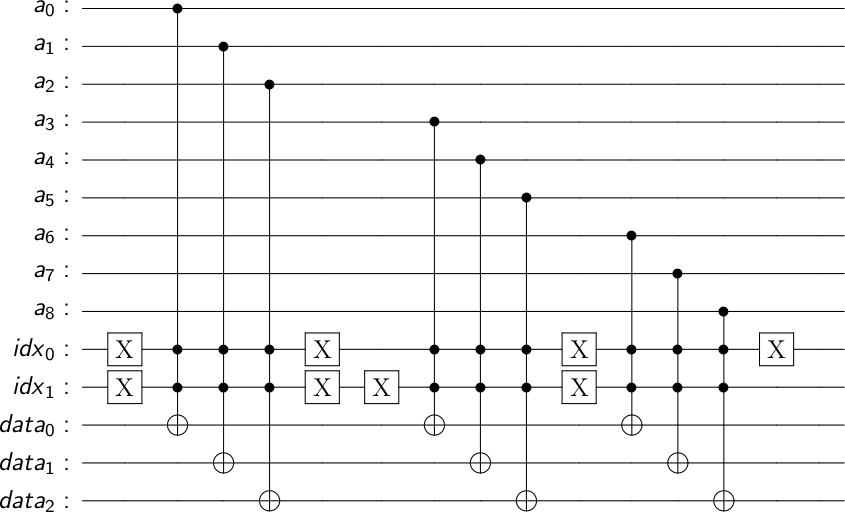
\includegraphics[scale=0.5]{../paper/results/indexer_3x3.png} 
      \caption{Indexer Circuit for a $3 \times 3$ matrix}
      \label{fig:indexer_circuit_3x3}
    \end{figure}
    \end{column}
    \begin{column}{0.5\colwidth}
      \vfill
      The role of the indexer is to output $A[i]$, where $A$ is an $m \times n$
      matrix and $i$ is an integer index. 

      \vspace{1em}

      We encode the matrix $A$ using $size(A)$ qubits, where $size(A)$ is the
      total number of elements in $A$.  The integer index is encoded using
      $log_2(m)$ qubits in the binary format.
    \end{column}
  \end{block}

  \begin{block}{Inner Product circuit}
    \begin{column}{0.5\colwidth}
    \begin{figure}
      \centering
      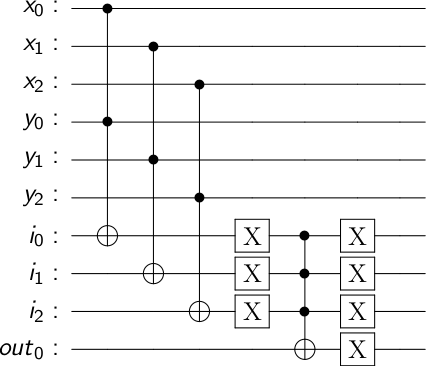
\includegraphics[scale=0.7]{../paper/results/inner_product_3x1.png} 
      \caption{Inner Product Circuit for $3 \times 1$ vectors}
      \label{fig:inner_product_circuit_3x1}
    \end{figure}
    \end{column}
    \begin{column}{0.5\colwidth}
      \vfill
      The inner product circuit \ref{fig:inner_product_circuit_3x1}, as the name
      suggests, computes the inner product between two vectors encoded as
      qubits.
      
      \vspace{1em}

      Our implementation only handles binary numbers (where
      multiplication is defined as logical $AND$ and addition as logical $OR$),
      but can be easily extended to support other data types.
    \end{column}
  \end{block}

  \begin{block}{QVMP Marking Oracle}
    \begin{figure}
  \centering
  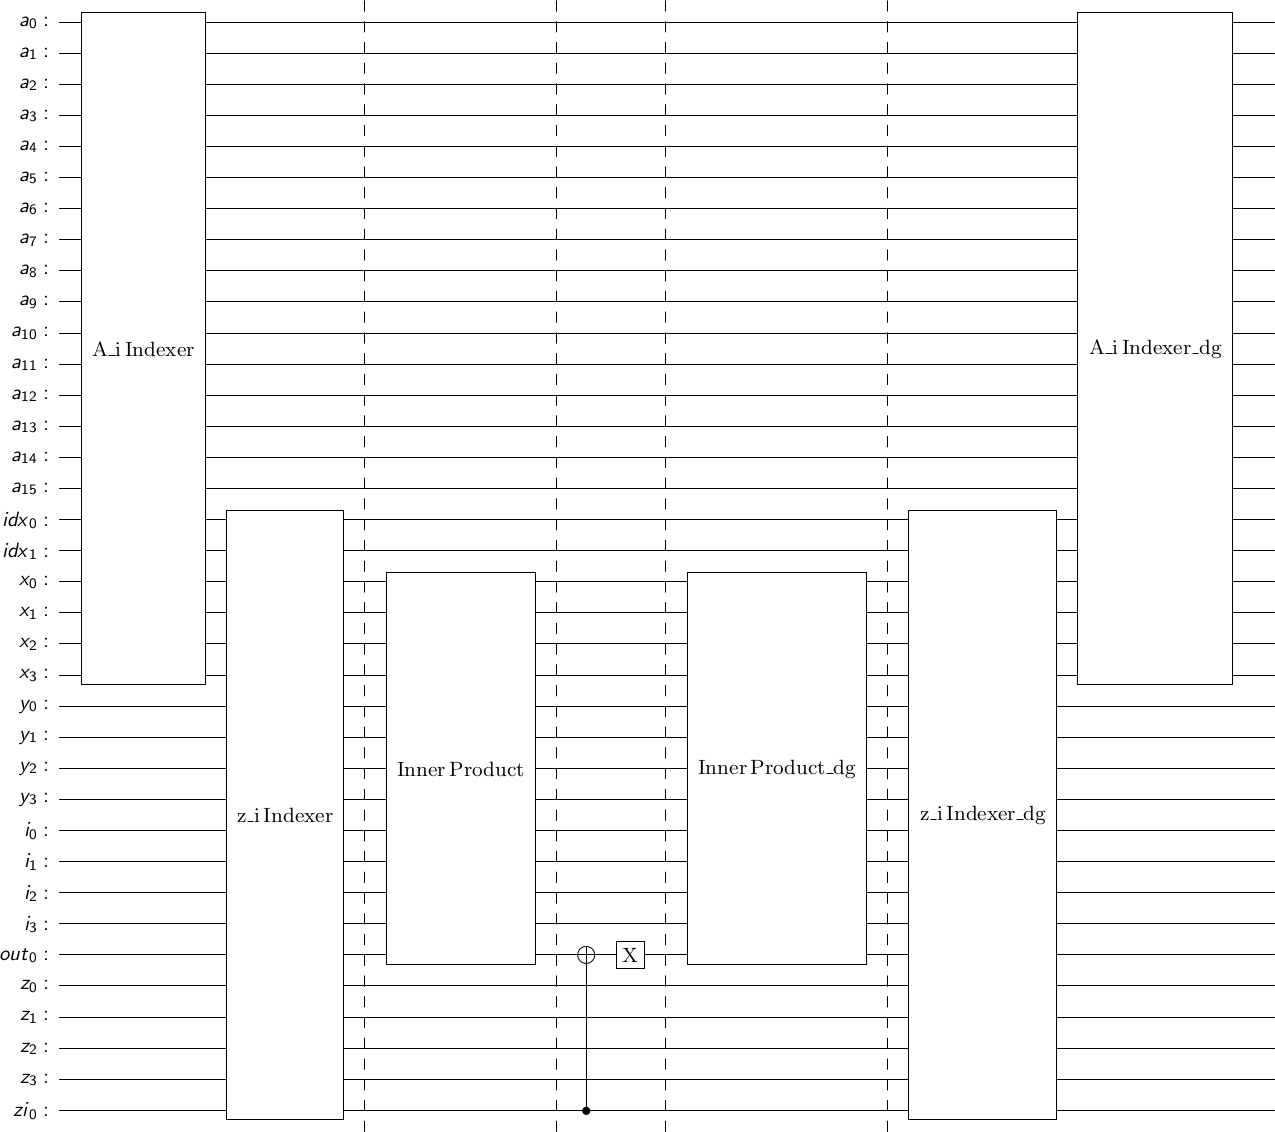
\includegraphics[scale=0.5]{../paper/results/oracle_circuit_4x4.png} 
  \caption{QVMP Marking Oracle for a $4 \times 4$ matrix}
  \label{fig:marking_oracle_4x4}
\end{figure}
  \end{block}
\end{column}

\separatorcolumn

\begin{column}{\colwidth}
  \begin{block}{Metrics}
    \begin{table}[t]
      \centering
      \begin{tabular}{c r}
       \toprule
        \textbf{Order of matrix} & \textbf{Time (in seconds)} \\
       \midrule
        2 & 0.24 \\
        4 & 0.81 \\
        8 & 2.38 \\ 
        16 & 27.48 \\
        24 & 66.20 \\
        \bottomrule
      \end{tabular}
      \caption{VMP Circuit Transpilation Stats}
      \label{table:transpilation_stats}
    \end{table}

    \begin{table}[t]
      \centering
      \begin{tabular}{c r r r}
        \toprule
        \textbf{Order of matrix} & \textbf{Total Gates} & \textbf{Circuit
        Depth} & \textbf{Qubit Count} \\
        \midrule
        2 & 269 & 94 & 15 \\
        4 & 1131 & 415 & 36 \\
        8 & 3164 & 1255 & 101 \\
        16 & 30740 & 13445 & 326 \\
        24 & 63193 & 28581 & 679 \\
        32 & 130960 & 60564 & 1159 \\
        \bottomrule
      \end{tabular}
      \caption{VMP Circuit Stats}
      \label{table:circuit_stats}
    \end{table}

  \end{block}

  \begin{block}{Future Work}
    \begin{itemize}
      \item \textbf{Optimize for space complexity}: Our current
        implementation uses a naive encoding of matrices which can be quite
        wasteful since most of the qubits are not used for the rest of the
        computation within the oracle. We can use quantum multiplexers like
        QRAM \cite{qram_2008} to achieve a quadratic improvement in space
        complexity.
      \item \textbf{Investigate automatic synthesis of Grover oracles}:
        Implementing quantum oracles by hand is challenging. Matters become
        more complicated when entanglement gets involved. Further,
        hand-tuning for space-complexity while maintaining correct can get
        tricky. We can approach this problem by developing compilers that
        automate the synthesis of reversible oracles from high-level
        classical descriptions. To encorporate verification, we either
        develop our compiler within existing formal verification frameworks
        like VOQC \cite{voqc_2021} or target standard formats like OpenQASM which can then be
        consumed by formally-verified optimizers. Quipper
        \cite{quipper_2013} and REVS \cite{amy2017verified} have made strides in this direction
    \end{itemize}
  \end{block}

  \begin{block}{References}

    \nocite{*}
    \footnotesize{\bibliographystyle{plain}\bibliography{poster}}

  \end{block}

\end{column}

\separatorcolumn
\end{columns}
\end{frame}

\end{document}
